%!TEX program = xelatex

% \documentclass[notes]{beamer}
% \documentclass[notes=only]{beamer}
\documentclass{beamer}

% Good bibliography
\RequirePackage[backend=biber]{biblatex}
\addbibresource[datatype=bibtex]{biblio.bib}

% Icon Fonts
\RequirePackage{academicons}
\RequirePackage{fontawesome}

% Correct the path when including svg pictures
\RequirePackage{import}

% For nice verbatim
\RequirePackage{minted}

% To resize graphic and table
\RequirePackage{graphics}

% For captions
\RequirePackage{caption}

% Arrange theme
\usetheme[
	progressbar=frametitle,
	sectionpage=none,
	numbering=fraction
]{metropolis}

% Color the progress:
% - green for SciLifeLab
% - violet for KI
\setbeamercolor{progress bar}{fg=violet,bg=white}

\author{\faUser\ Maxime Garcia\\ \faTwitter\ \href{https://twitter.com/gau/}{@gau}\\ \faGithub\ \href{https://github.com/MaxUlysse/}{@MaxUlysse}\\ \faGlobe\ \href{https://maxulysse.github.io/}{maxulysse.github.io}}
\date{2018-02-26}
\title{Presenting Sarek}
\titlegraphic{\hfill
\includegraphics[height=1cm]{pictures/Sarek_no_border}}
\subtitle{Formerly known as CAW}
\institute{SciLifeLab NGI / BarnTumörBanken\\ % Don't forget logos
	\vfill
	
\includegraphics[height=.7cm]{pictures/SciLifeLab}
	\hfill
	
\includegraphics[height=.7cm]{pictures/NGI}
	\hfill
	
\includegraphics[height=.7cm]{pictures/NBIS}
	\hfill
	
\includegraphics[height=.7cm]{pictures/KI}
	\hfill
	
\includegraphics[height=.7cm]{pictures/KTH}
	\hfill
	
\includegraphics[height=.7cm]{pictures/SU}
	\hfill
	
\includegraphics[height=.7cm]{pictures/UU}
	\hfill
	
\includegraphics[height=.7cm]{pictures/Barntumorbanken}
}

\begin{document}

\maketitle

\section{From CAW to Sarek}

\begin{frame}{CAW}
	\begin{center}
		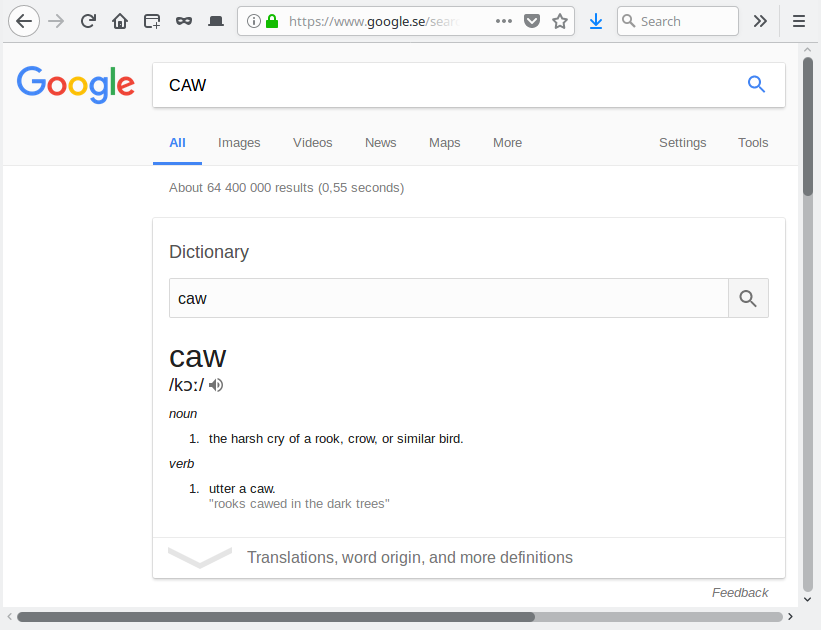
\includegraphics[height=7cm]{pictures/Definition.png}
		\captionof*{figure}{What happens when you look for CAW}
	\end{center}
\end{frame}

\begin{frame}{Sarek}
	\begin{center}
		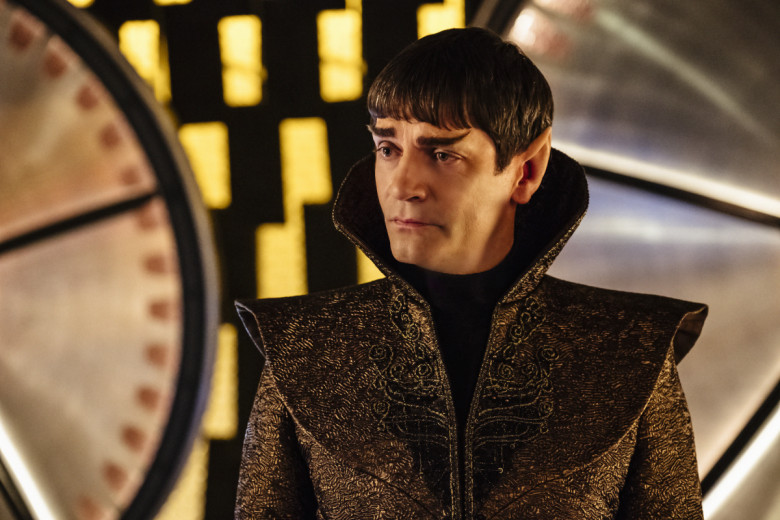
\includegraphics[height=7cm]{pictures/Sarek_discovery.jpg}
		\captionof*{figure}{James Frain as Sarek, "Star Trek: Discovery"}
	\end{center}
\end{frame}

\begin{frame}{The real inspiration}
	\begin{center}
		\includegraphics[height=7cm]{pictures/Skierfe-summer.jpg}
		\captionof*{figure}{Mount Skierfe in the Sarek National Park in Summer}
	\end{center}
\end{frame}

\begin{frame}{How it should look today}
	\begin{center}
		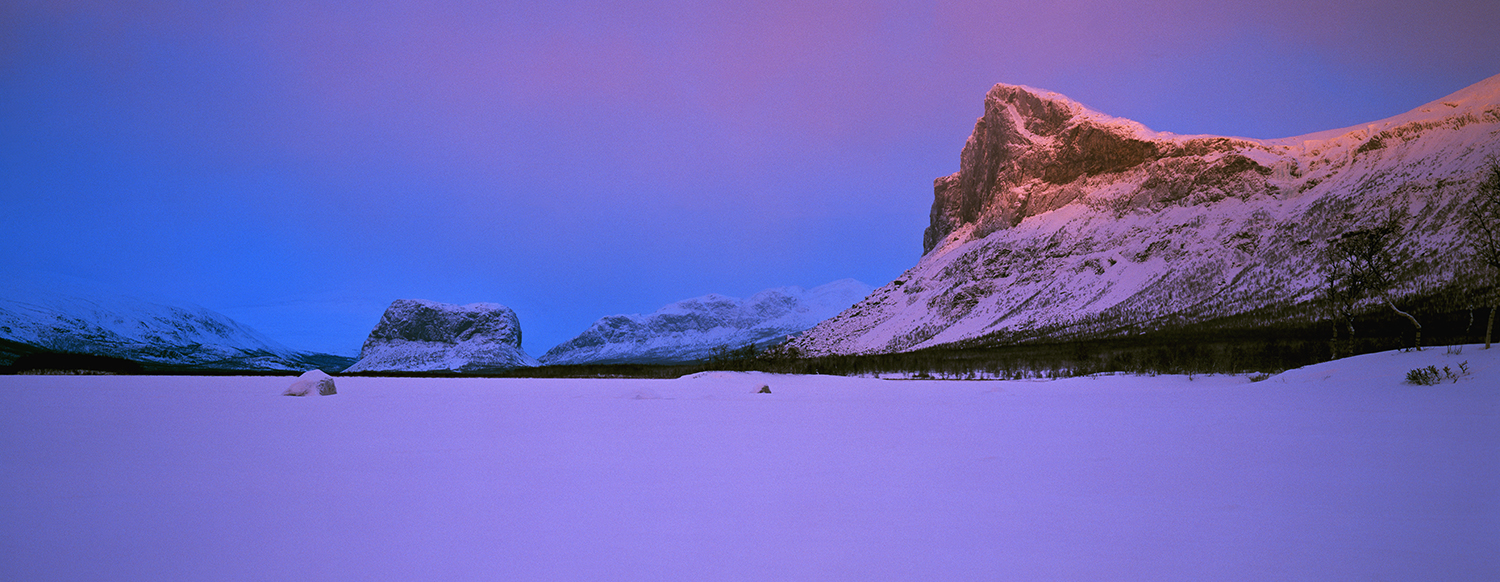
\includegraphics[height=4cm]{pictures/Skierfe-winter.jpg}
		\captionof*{figure}{Mount Skierfe in Winter}
	\end{center}
\end{frame}

\begin{frame}{What does Sarek do?}
	\begin{center}
		
\includegraphics[height=1cm]{pictures/Sarek}
	\end{center}
	\pause
	\begin{center}
		
\includegraphics[height=1cm]{pictures/Sarek_germline}
	\end{center}
	\pause
	\begin{center}
		
\includegraphics[height=1cm]{pictures/Sarek_somatic}
	\end{center}
\end{frame}

\section{Acknowledgments}

\begin{frame}{The List of People Involved}
	\begin{table}
		\resizebox{.8\textwidth}{!}{%
		\begin{tabular}{ll}
			Sebastian DiLorenzo &	Markus Mayrhofer \\
			Jesper Eisfeldt 		&	Monica Nistèr \\
			Phil Ewels					& Björn Nystedt \\
			Maxime Garcia 			&	Pall Olason \\
			Szilveszter Juhos 	&	Markus Ringnér \\
			Max Käller 					&	Pelin Sahlén \\
			Malin Larsson 			&	Johanna Sandgren \\
			Marcel Martin 			&	Teresita Díaz De Ståhl \\
		\end{tabular}}
	\end{table}
\end{frame}

\begin{frame}{Where to find us?}
	\begin{itemize}
		\item We are on the SciLifeLab Slack

		\faSlack\ \href{https://scilifelab.slack.com/}{\#cancer-pipeline}
		\pause
		\item We have a gitter channel

		\faGroup\ \url{https://gitter.im/SciLifeLab/Sarek}
		\pause
		\item Our code is hosted on Github

		\faGithub\ \url{https://github.com/SciLifeLab/Sarek}
	\end{itemize}
\end{frame}


\usebackgroundtemplate{
	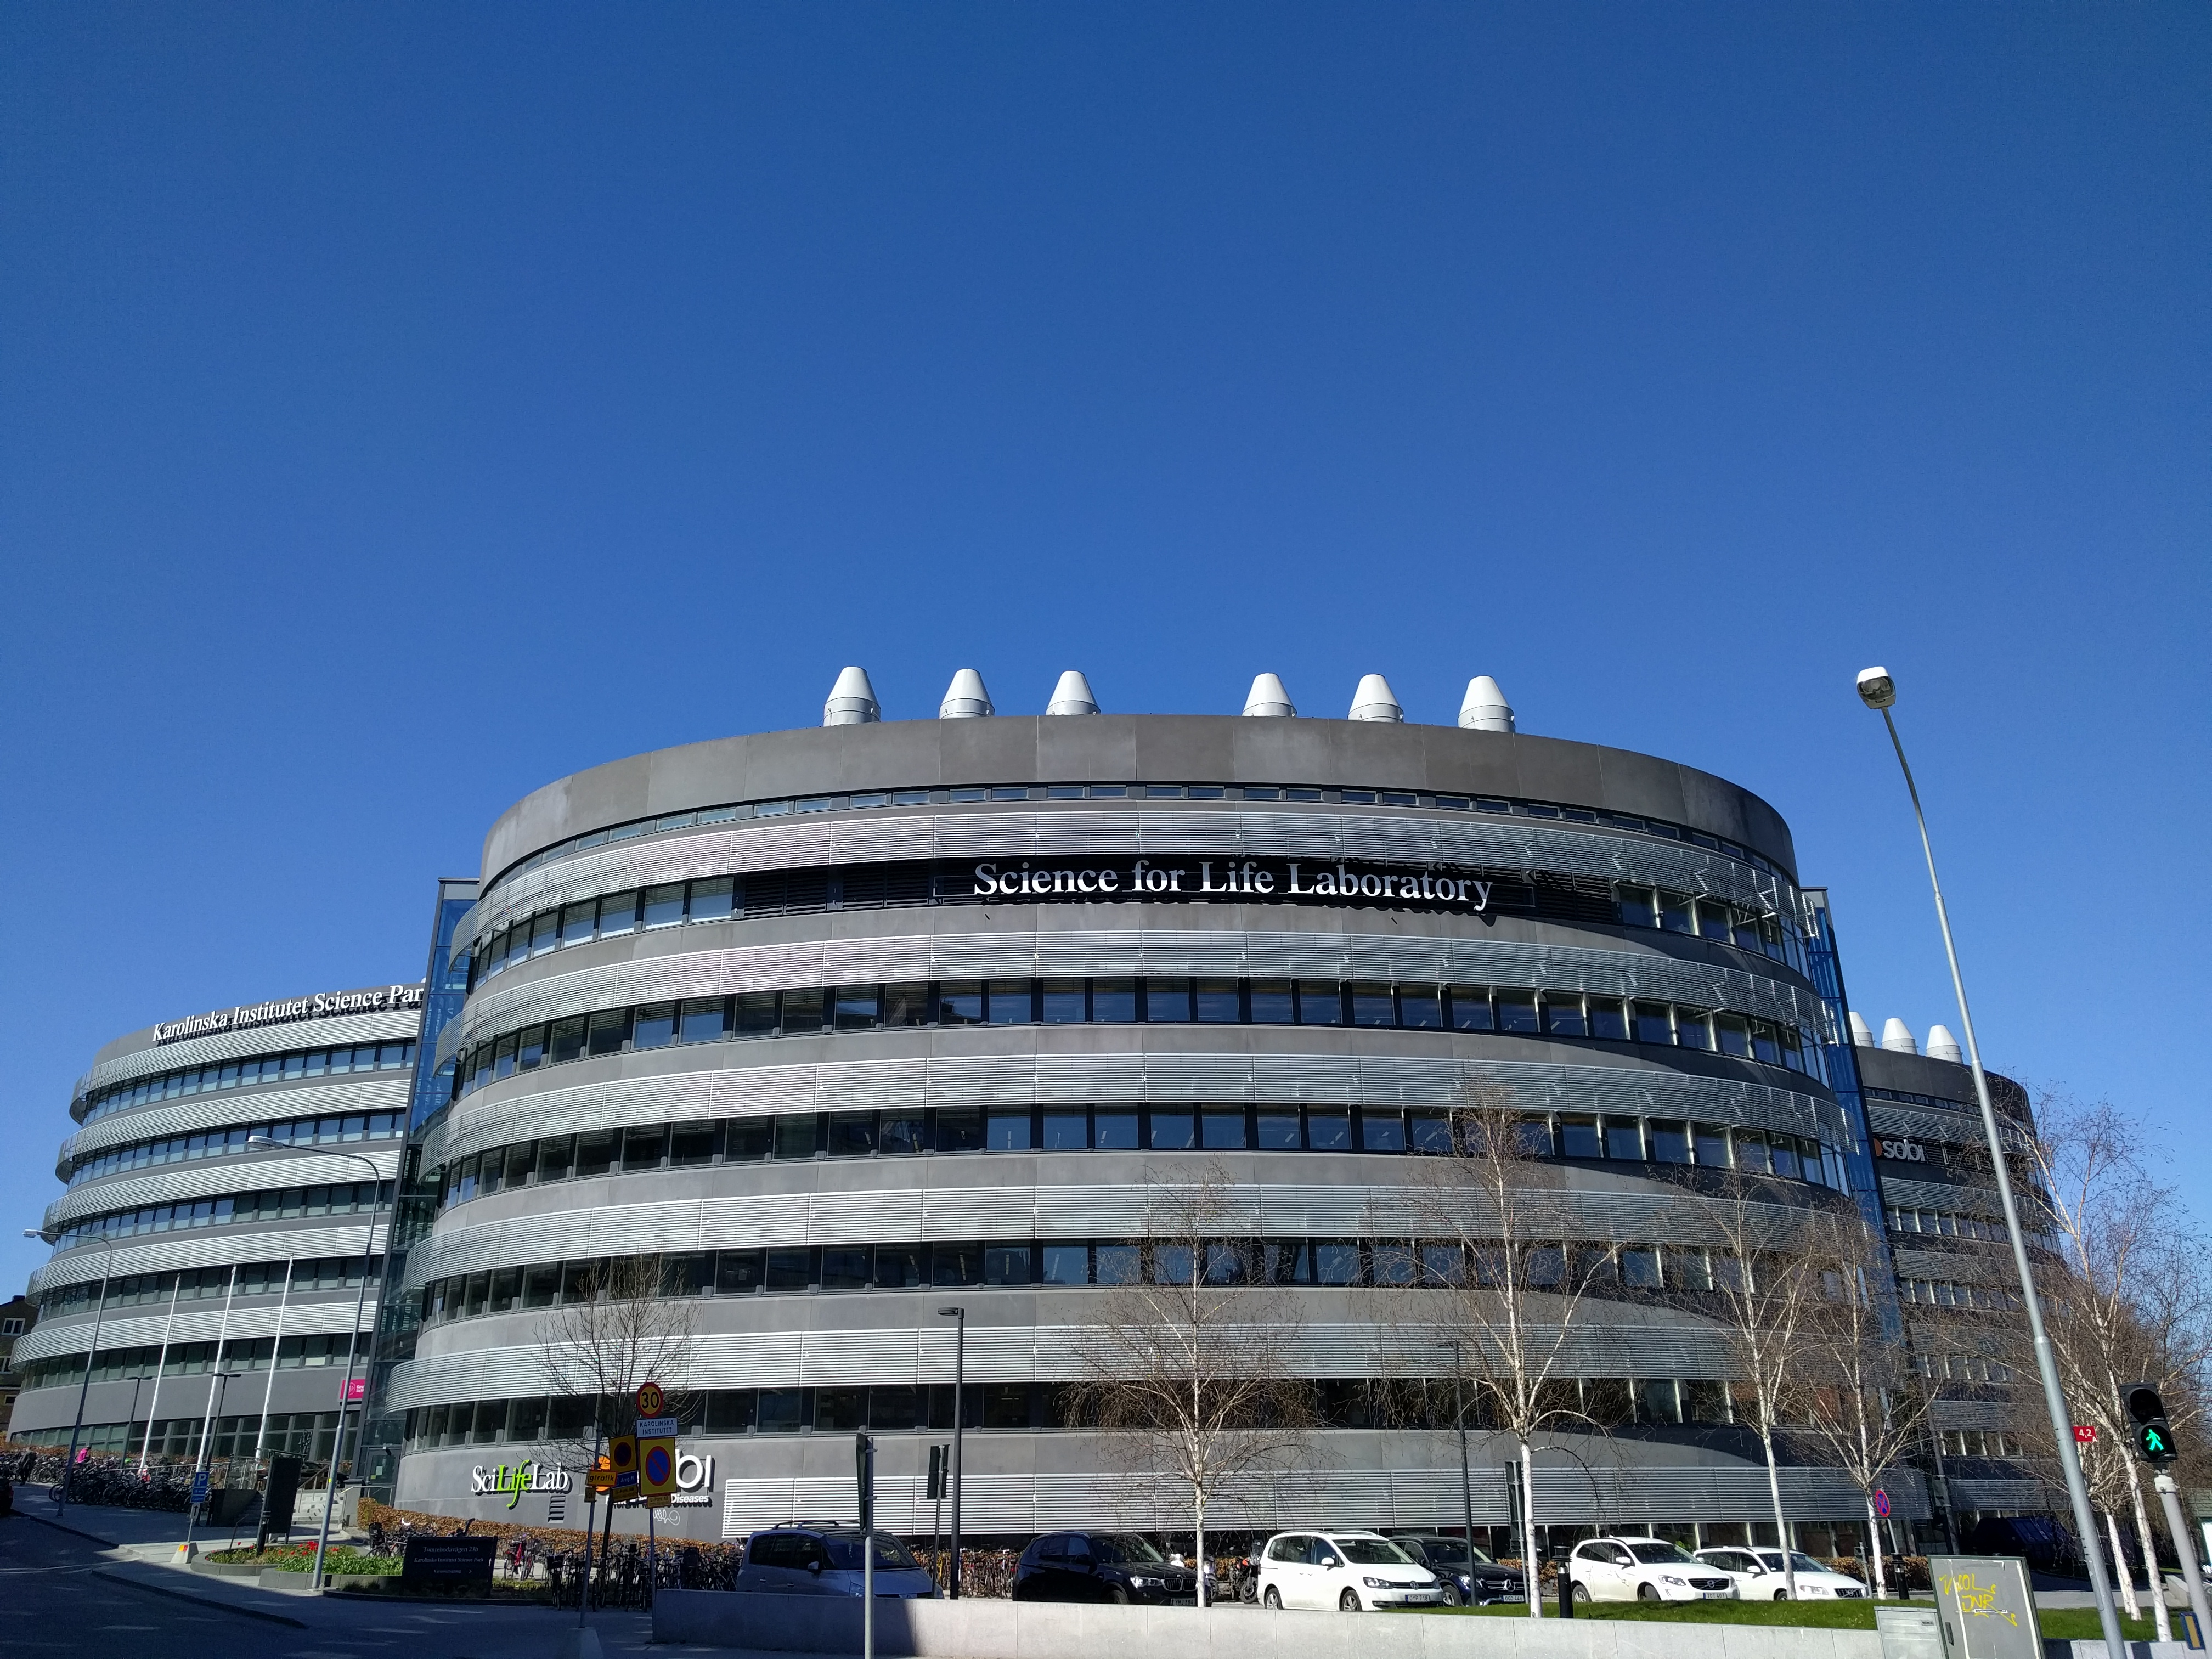
\includegraphics[width=\paperwidth]{pictures/SciLifelab-BlueSky.jpg}
}

\begin{frame}[plain,noframenumbering]{Any questions?}
\end{frame}

\end{document}
